\documentclass[12pt,a4paper]{article}
\usepackage{enumitem}
% Define margins
\setlength{\topmargin}{-1.0cm}
\setlength{\oddsidemargin}{0.1cm}
\setlength{\textwidth}{16.5cm}
\setlength{\textheight}{23.0cm}

% Use Times New Roman font
\usepackage{times}
\usepackage{xurl}
\usepackage{url}
\usepackage[hidelinks]{hyperref} 
\usepackage{amsmath} 
\urlstyle{rm}

\renewcommand{\rmdefault}{ptm}

\usepackage{graphicx} % LaTeX package to import graphics
\graphicspath{{images/}} % Configuring the graphicx package

% Define header and footer
\usepackage{fancyhdr}
\pagestyle{fancy}
\fancyhf{}
\cfoot{\textbf{\textit{\thepage}}}
\renewcommand{\headrulewidth}{0.7pt}
\setlength{\headheight}{14pt}

% Adjust section and subsection title formats
\usepackage{titlesec}
\titleformat{\section}
  {\normalfont\fontsize{14}{15}\bfseries}{\thesection}{1em}{}
\titleformat{\subsection}
  {\normalfont\fontsize{12}{15}\bfseries}{\thesubsection}{1em}{}

% Define a style with no footer for the table of contents
\fancypagestyle{nofooter}{%
  \fancyfoot{}%
}

% To manage references
\usepackage{natbib}
\usepackage[labelfont=bf]{caption}

\begin{document}

% TITLE PAGE

\begin{titlepage}

\newcommand{\HRule}{\rule{\linewidth}{0.5mm}}
\center

\vspace*{1\baselineskip}

\includegraphics[width=0.15\textwidth]{images/UTS.png}\\
\textsc{\LARGE University of Technology Sydney}\\[2.0cm]
\textsc{\Large (32557) Enabling Enterprise Information Systems}\\[0.4cm]

\HRule\\[0.6cm]
{\huge\bfseries Design Thinking \& IS-Enabled Solutions (Part 2) }\\[0.4cm]
\HRule\\[10cm]

\emph{by Team Super} \\
{ Seoyoon Kim (25388442) [Group leader] \\}
{ Jin Lee (25388733)  \\}
{ Ariel Manueke (25207919) \\}
{ Nonthawat Praisompong (25233750) \\}

\vfill
{\large\today}

\vfill

\end{titlepage}

% TABLE OF CONTENTS

\tableofcontents
\thispagestyle{nofooter}
\cleardoublepage

\pagebreak

% DOCUMENT CONTENT STARTS HERE
% You can start writing your document content here.


% Student %%%%%%%%%%%%%%%%%%%%%%%%%%%%%%%%%%%%%%%%%%%%%%%%%%%%%%%%%%%%%%%%%%%%%%%%%%%%%%%%%%%%%%%%%

\setcounter{page}{1}

\section{Question 1}
\subsection{Uber Trip Journey Map Activity} 

\begin{figure}[htbp]
    \centering
    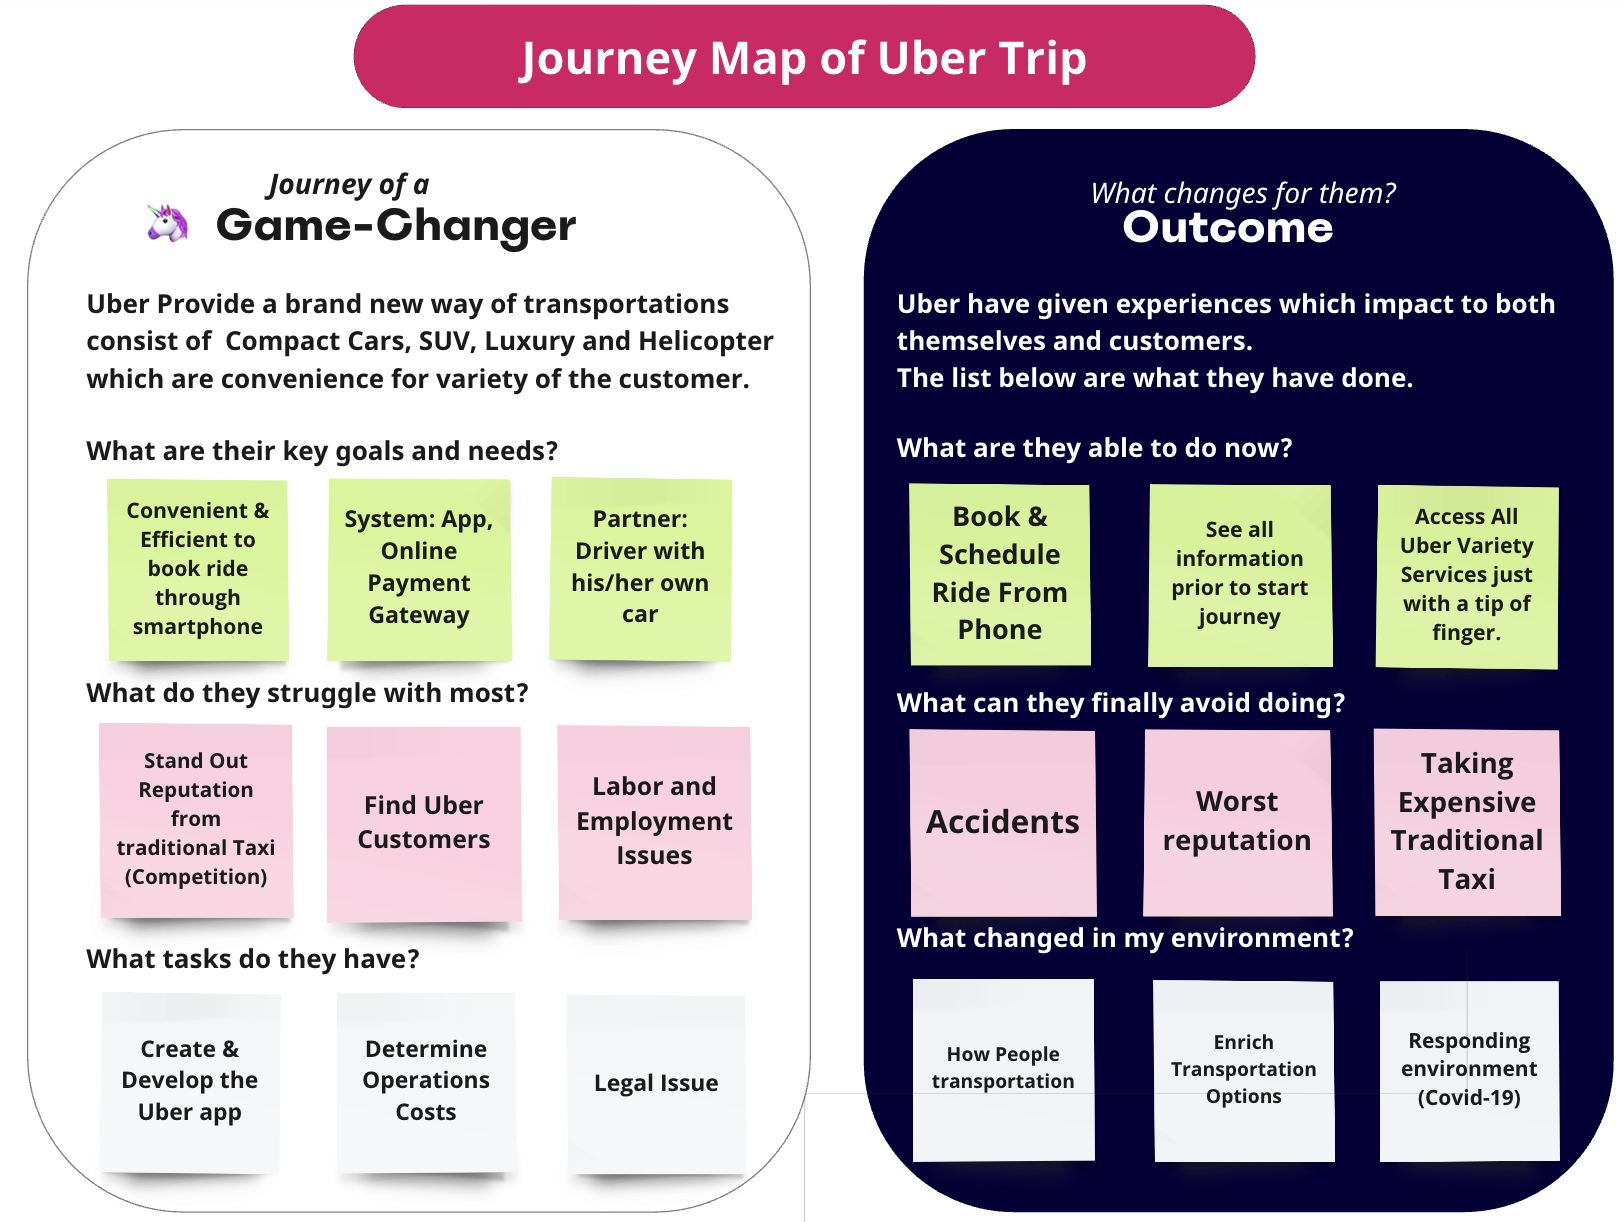
\includegraphics[width=1\textwidth]{images/Journey1.png}\
    \caption{Journey Map Identification}
    \label{fig:example}
\end{figure}

\text{Both Figure 1 and Figure 2 are made based on \cite{Ref1.1}.}

\begin{figure}[htbp]
    \centering
    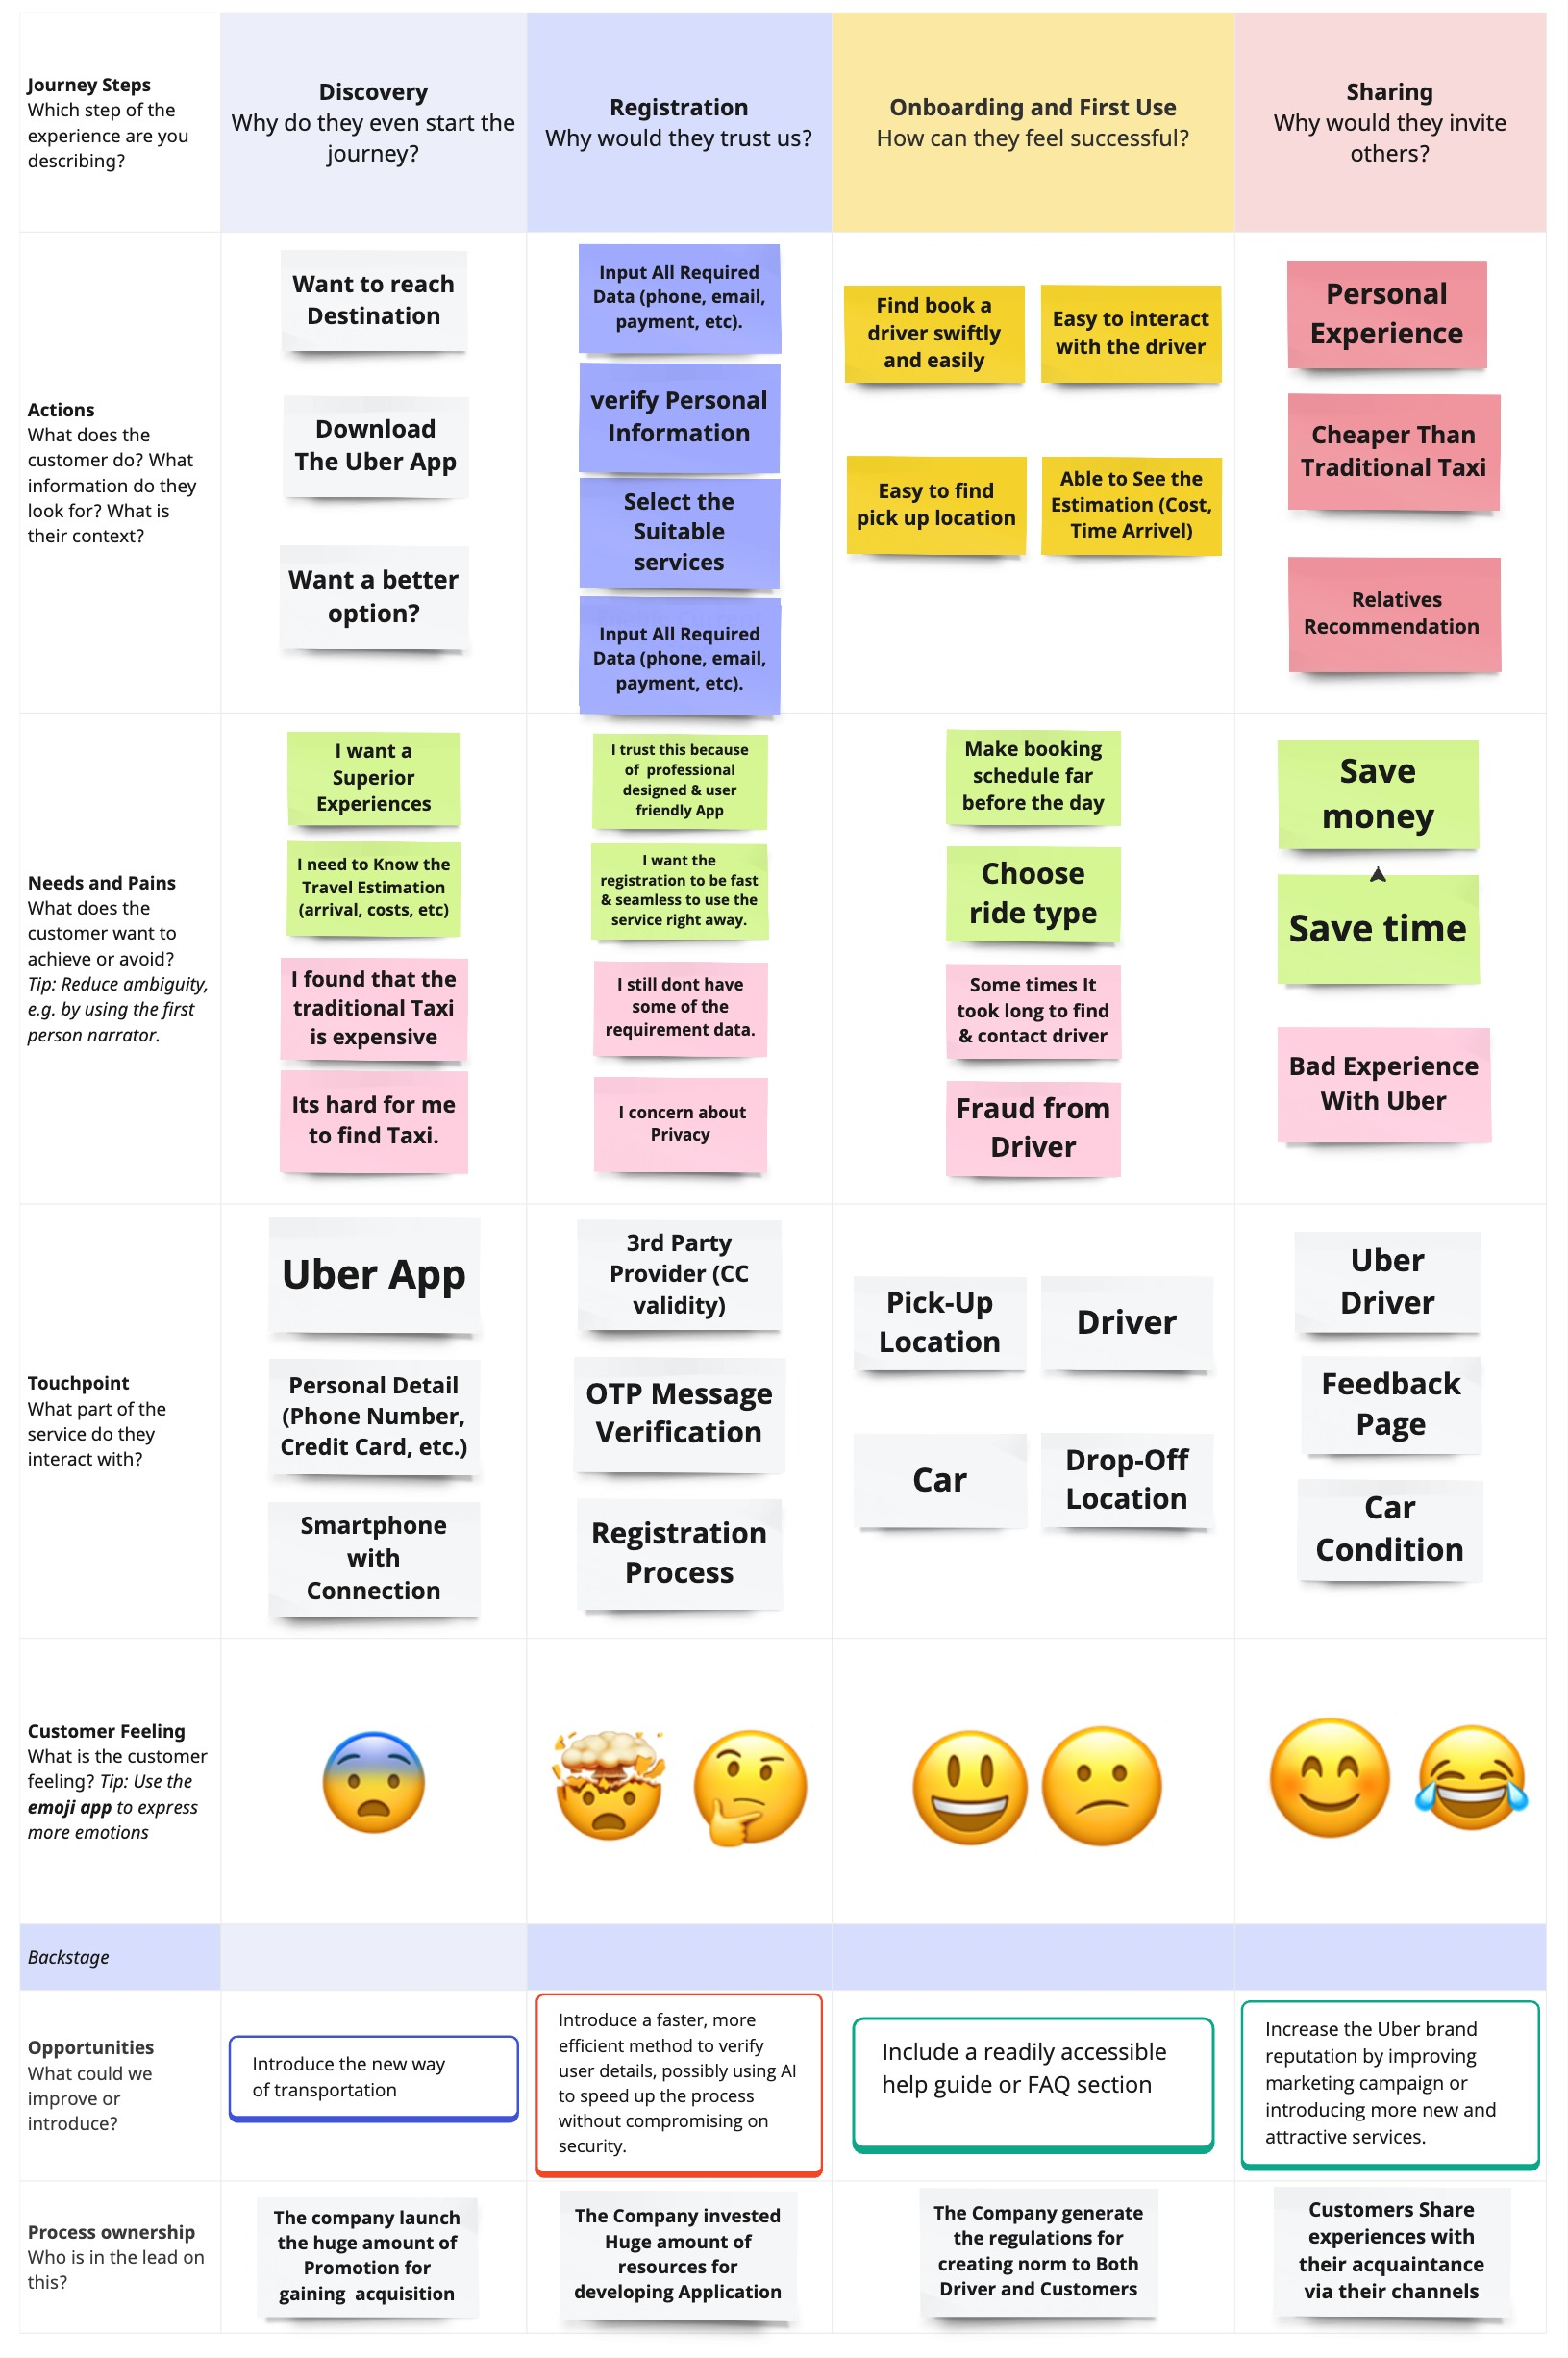
\includegraphics[width=0.88\textwidth]{images/Journey2.jpg}\
    \caption{Journey Map Table}
    \label{fig:example}
\end{figure}

\pagebreak%%%%%%%%%%%%%%%%%%%%%%%%%%%%%%%%%%%%%%%%%%%%%%%%%%%%%%%%%%%%%%%%%%%%%%%%%%%%%%

\setcounter{page}{3}

\section{Question 2}
\subsection{Joint Value Proposition for a Mental Health Web Tool}
\label{sec:Question 2}

\begin{figure}[htbp]
    \centering
    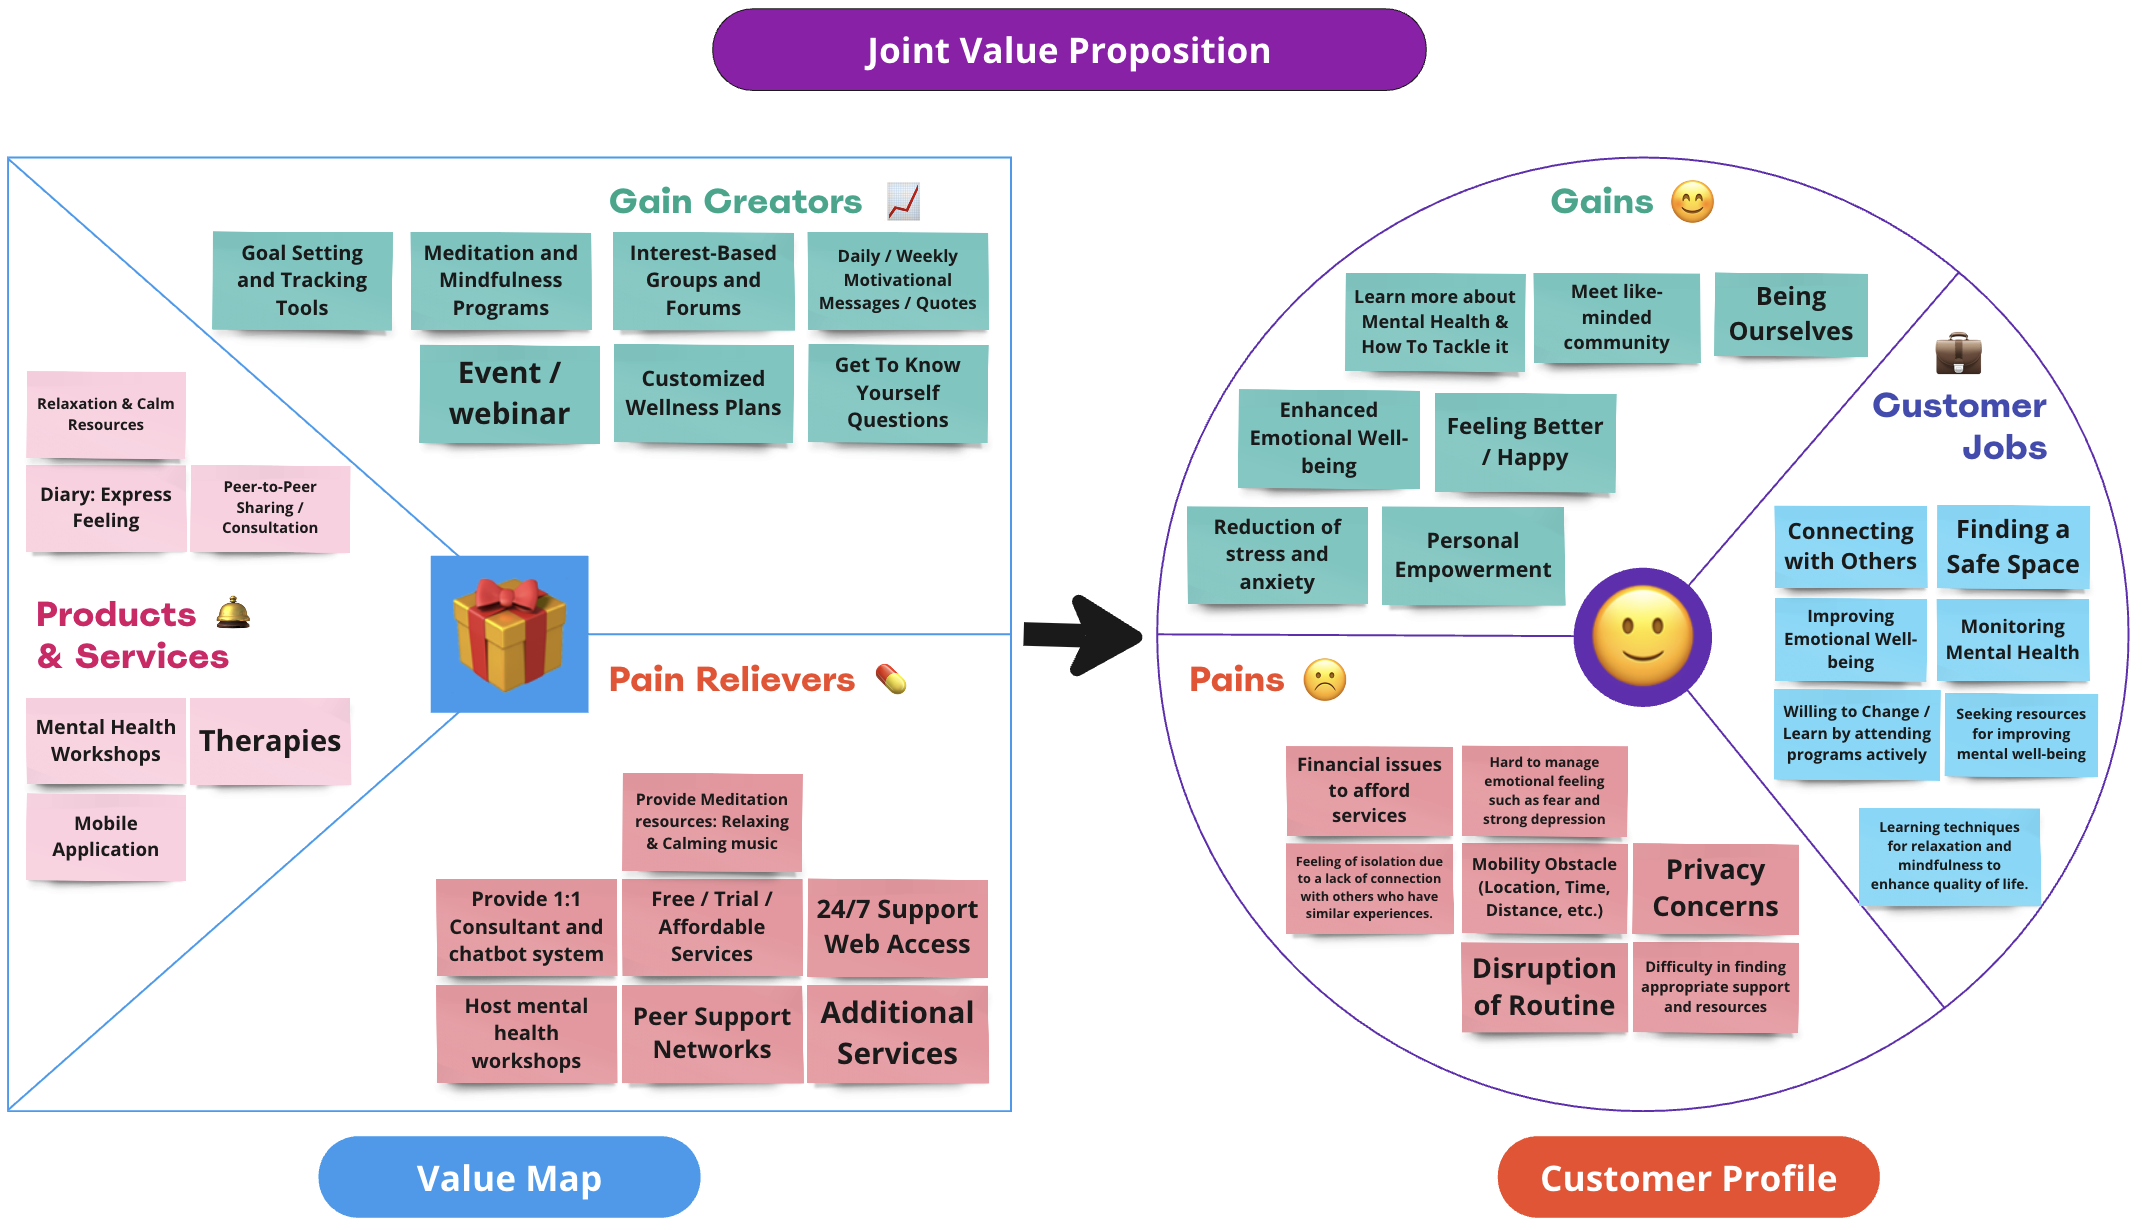
\includegraphics[width=1\textwidth]{images/JointValue.png}
    \caption{Joint Value Proposition Canvas}
    \label{fig:example}
\end{figure}

\noindent\text{This diagram is made based on \cite{Ref2.1}.}


\pagebreak
%%%%%%%%%%%%%%%%%%%%%%%%%%%%%%%%%%%%%%%%%%%%%%%%%%%%%%%%%%%%%%%%%%%%%%%%%%%%%%

\setcounter{page}{4}

\section{Question 3}
\subsection{Level-2 Lotus Blossom Diagram for Qantas Service/Product Ideation}
\label{sec:Question 3}
\begin{figure}[htbp]
    \centering
    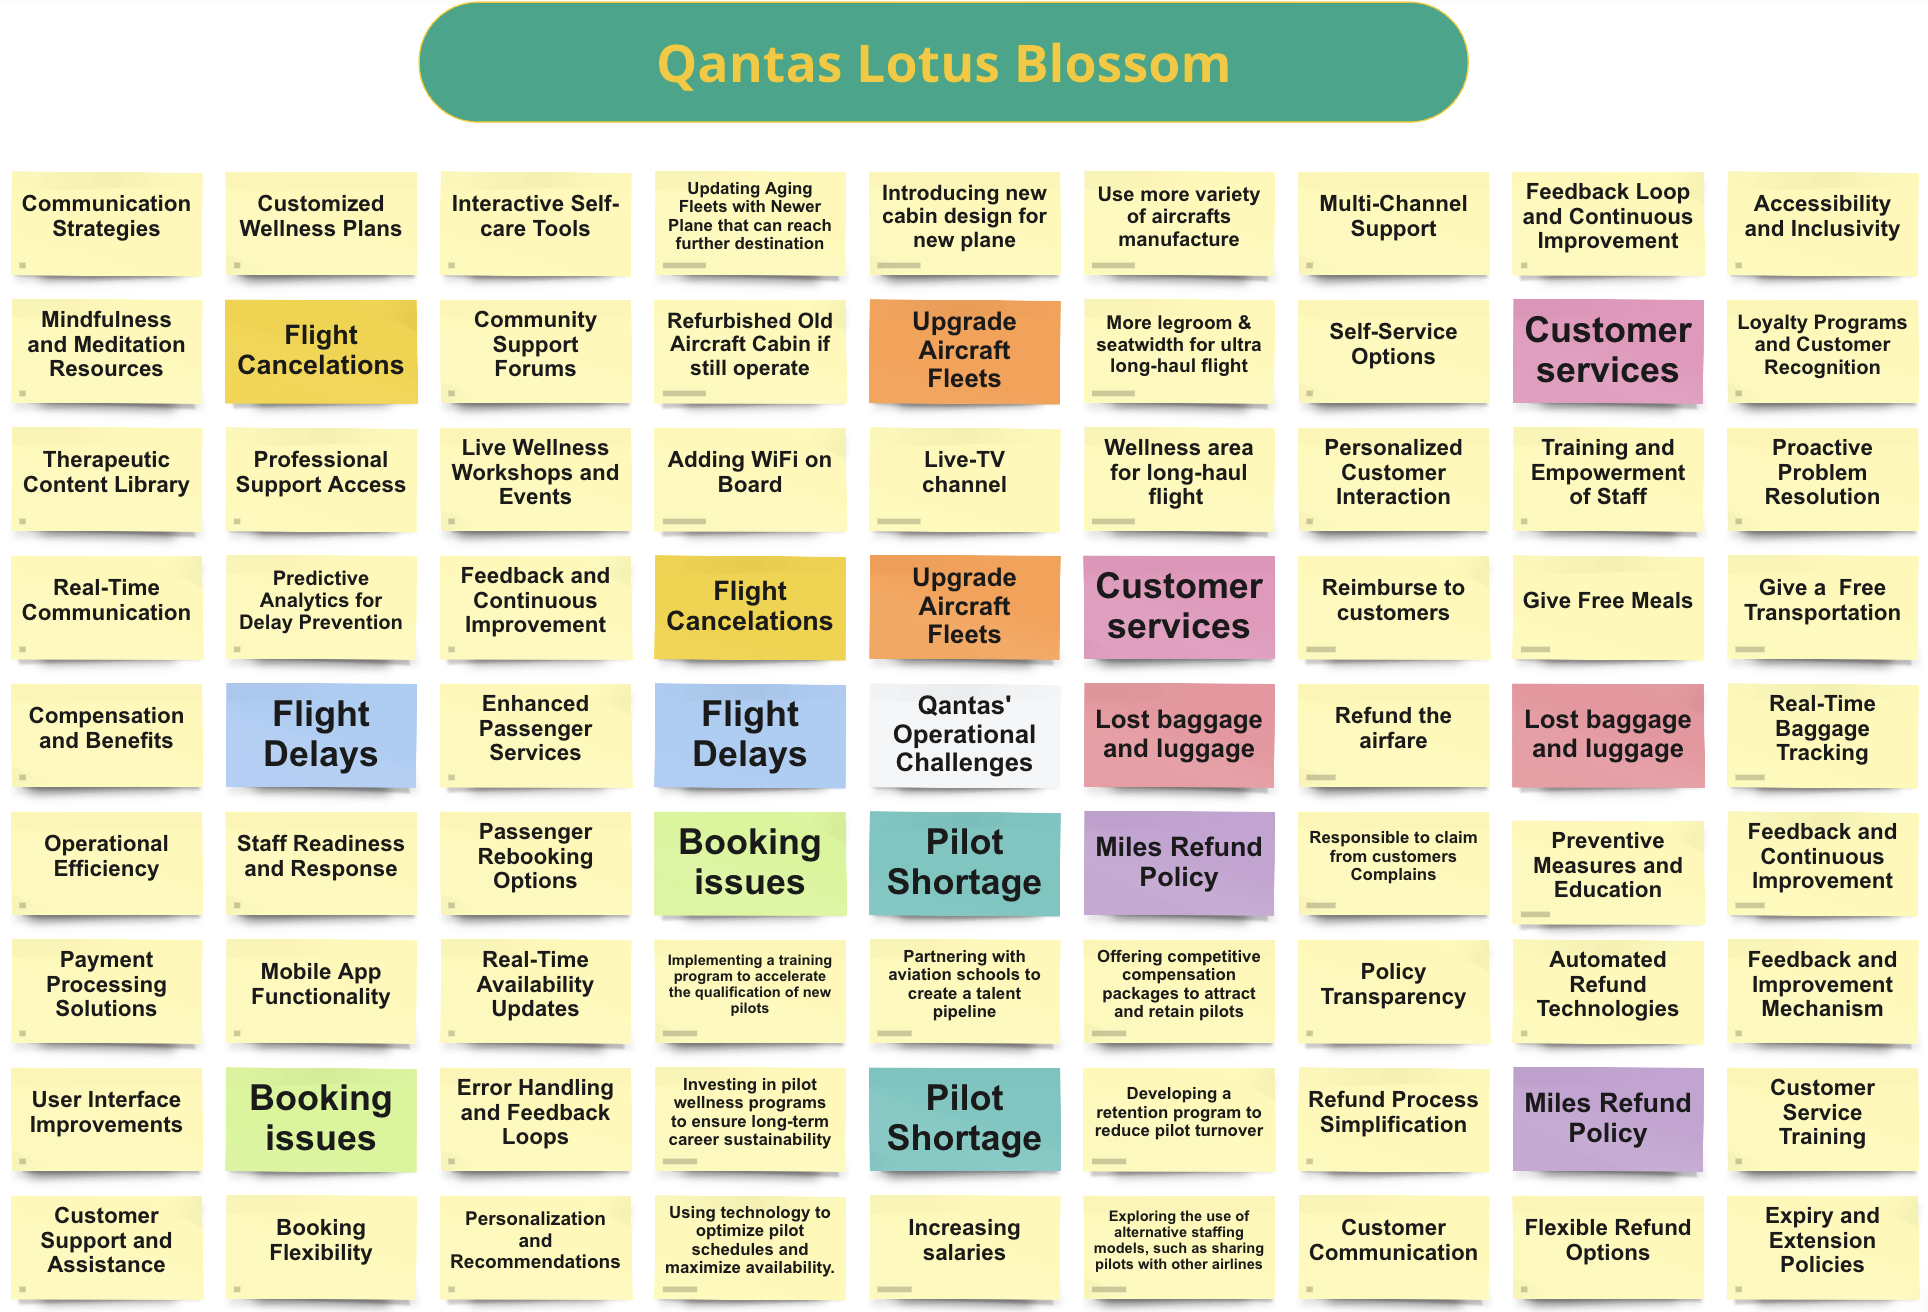
\includegraphics[width=1.0\textwidth]{images/Lotus Blossom.png}
    \caption{Empathy Map Result}
    \label{fig:example}
\end{figure}
This image is made based on:\\
\begin{itemize}
    \item \cite{Ref3.1}.
    \item \cite{Ref3.2}.
    \item \cite{Ref3.3}.    
\end{itemize}

\pagebreak
% BIBLIOGRAPHY %%%%%%%%%%%%%%%%%%%%%%%%%%%%%%%%
 

% Use Leeds Harvard referencing template
\bibliographystyle{lsharvard}
% Add here the bib file with your references
\bibliography{references}
	
\def\UrlBreaks{\do\/\do-}

\clearpage
\end{document}
